\section{Our Approach}
Our initial approach is inspired by similar sound recognition problems and
existing methods.
Such problems include the recognition of voice, music, and animal vocalisations
of species other than birds.
It is observed that these problems, while similar in nature, differ in practice.
This is mainly due to the nature of the sound being analysed, as well as
domain knowledge of the structure.

For example, the structure of human voice is well studied, and patterns are
easily automatically identified today.
Specialised methods for modelling and analysing voice recordings exist, such as 
hidden markov models, dynamic time warping, neural networks.
Human speech recognition is however a different task entirely, as the goal here
is to identify words, and not the individual speaking.
One could consider the problem of individual identification, which may provide
insight into useful methods.

Music recognition is trivial in the case of identifying pure reproductions,
the main challenge in this area being noise reduction and distortion compensation.
Music can be easily identified using statistical methods to compare pitch
variations along the duration of the recording.
Bird song however contains many variations and transpositions within the same
species which make it difficult to find an archetypal sequence of pitch
variations.
The issue of noise reduction remains relevant to our problem.\\

A common approach to solving these problems is to first reduce it to an image
recognition problem by using the spectrographic representation of the audio.
Elements descriptive of specific labels are searched for within a the
spectrogram of a target example.
The simplicity and success of such solutions has driven the direction of this
project.

Our approach uses a combination of computer vision and machine learning
techniques to construct a fully automatic recognition system.
Standard image processing methods are used to process spectrograms and extract
sections of song which may be used to identify a particular species, much like
how an orthonologist visually inspects the song spectra.
These sections are then matched against new samples to be classified through a
multi-class machine learning algorithm.

\subsection{Process Overview and Document Outline}
The project is divided into four discrete parts, which follow the logical flow
of data in the system.
Each part is detailed in their relevant sections, including discussion on
possible alternatives and improvements to the mechanisms that have been
developed.
\begin{enumerate}
  \item \textbf{Collection:}
    Data is sourced from field recordings done in uncontrolled environments.
    The variety provides a good estimate of real-world performance and
    introduces many quality related issues.

  \item \textbf{Preparation and Selection:}
    Recordings are filtered and selected to maintain reasonable quality levels.
    Spectrograms are then derived from the recordings.
    This is now the representation that is used throughout the program until
    the feature vector is constructed.

  \item \textbf{Preprocessing and Feature Extraction:}
    Noise is reduced as much as possible to identify key regions of interest
    within the spectrogram image.
    These are extracted as templates and cross-correlated against other
    recording spectrograms to form a feature vector.

  \item \textbf{Classification and Evaluation:}
    The resulting data is then fed to a classifier and evaluated using techniques
    designed to reduce statistical bias.
\end{enumerate}

\subsection{Architectural Overview}

Flexibility is the primary concern in designing this system.
It is imperative that new processing and classification techniques are able to
be implemented and quickly evaluated.
Each stage is developed as a discrete stage in the system.
Figure~\ref{fig:sysoverview} describes the layout of the system by visualising
the flow of data.

Performance aspects are discussed as they appear in their relevant sections.
A summary of technologies and libraries used is available in Appendix~\ref{app:tech}.

Formal system and unit tests have not been written.
Given time the architecture could be concretised and test suites surely written.

\begin{figure}[!htb]
  \centering
  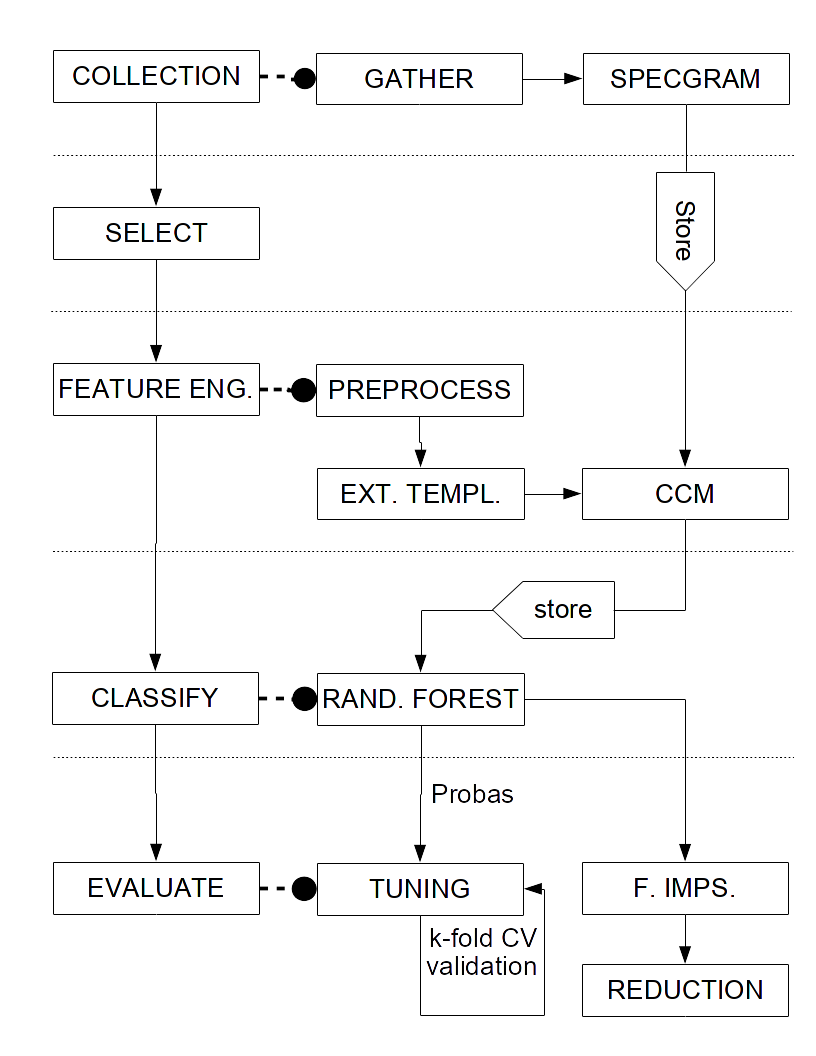
\includegraphics[width=1\textwidth]{block}
  \caption{System block diagram}
  \label{fig:sysoverview}
\end{figure}
